\begin{scanpage}{0122}{105}
the reflected signal equals zero if a whole number of half-waves $(l=\frac\lambda2n,\ n=1,2,3\ldots)$ is fitted into the length of the paraboloid, and it takes a maximum value if a half-integral number of half-waves $(l=\frac\lambda2(n+\frac12),\ n=1,2,3\ldots)$ is contained in this length.

A calculation performed by us on the basis of Equation (18.04) for paraboloids with the parameters $\Omega=90^\circ$, $\operatorname{tg}\omega=0.1$ $(k=\pi)$ shows (Figure 37) that, although the oscillating character of the effective scattering area is preserved, the amplitude of the oscillations is only 2 dB, and the maximum values of the function $\sigma$ exceed the corresponding values in the physical optics approach by almost 13 dB. A still stronger divergence between the results of our theory and physical optics is detected when the paraboloid is deformed into a disk (Figure 36, $ka=5\pi$, $k=\pi$, $\Omega=90^\circ$, $\omega\to90^\circ$).
\begin{center}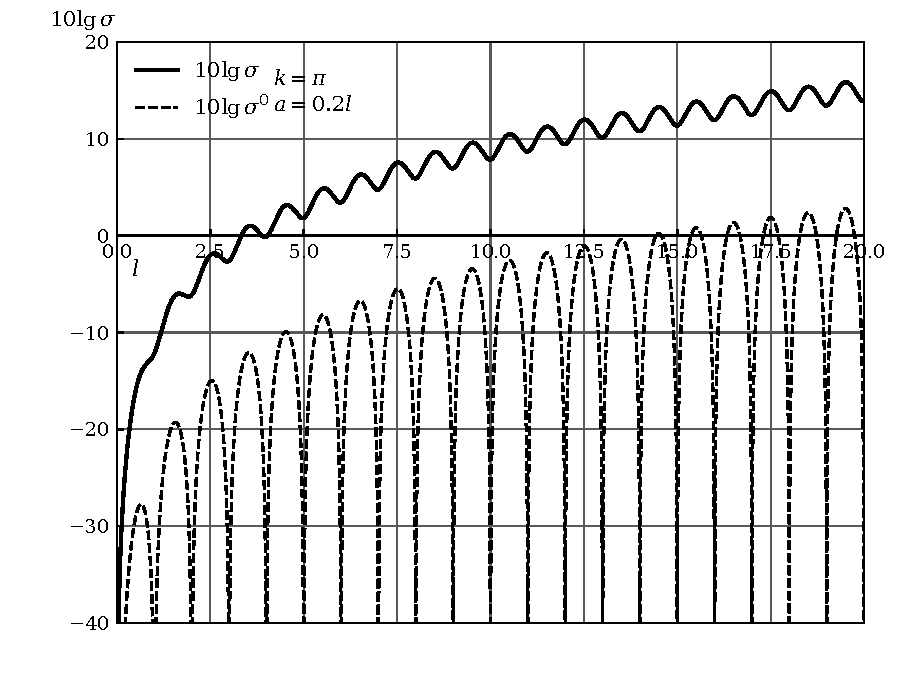
\includegraphics[width=.86\linewidth]{images/recreated/b-0122-fig37.pdf}

\begin{minipage}{.86\linewidth}Figure 37. The effective scattering area of a finite paraboloid as a function of its length with a constant value of the angle $\omega$ $(\operatorname{tg}\omega=0.1)$. The diameter of the base varies.\end{minipage}
\end{center}
\end{scanpage}
